% vim: set fileencoding=utf-8 encoding=utf-8:
\documentclass[spanish]{article}
\usepackage{babel}
\usepackage[utf8]{inputenc}
\usepackage{fullpage}
\usepackage{url}
\usepackage{palatino}
\usepackage{amsmath}
\usepackage{amssymb}
\usepackage{graphicx}


\title{Reconocimiento de Patrones \\
    Discusión del artículo \textit{Similarity~Measures}}
\author{Roberto Bonvallet \\ \url {<rbonvall@gmail.com>}}
\date{Agosto de 2008}

\begin{document}
\maketitle

% set members for next example
\newcommand{\SMA}{\Box}
\newcommand{\SMB}{\spadesuit}
\newcommand{\SMC}{\heartsuit}
\newcommand{\SMD}{\clubsuit}
\newcommand{\SME}{\diamondsuit}

\begin{align*}
    A &= \{\phantom{\SMA,  \SMB,} \SMC,          \SMD,          \SME\}  \\
    B &= \{\phantom{\SMA,} \SMB,  \SMC,          \SMD\phantom{, \SME}\} \\
    C &=          \{\SMA,  \SMB,  \SMC\phantom{, \SMD,          \SME}\} \\
\end{align*}

\begin{figure}
  \centering
  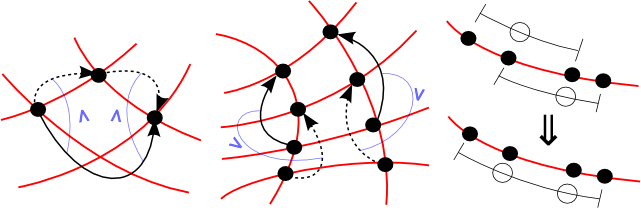
\includegraphics[bb=0 0 513 166]{imagenes/dom-cons-trans.png}
  % dom-cons-trans.png: 641x208 pixel, 90dpi, 18.09x5.87 cm, bb=0 0 513 166
  \caption{%
    Ejemplos de las propiedades de un espacio con estructura de proximidad
    monótona. Las líneas con flechas representan distancias entre puntos del
    espacio de características.
    (a) Dominancia: distancia diagonal es mayor que cada una de las distancias
        a lo largo de las dimensiones.
    (b) Consistencia: las relaciones de orden a lo largo de una dimensión son
        independientes de otras dimensiones.
    (c) Transitividad: relaciones de orden traslapadas fuerzan las mismas
        relaciones entre los puntos en la región de traslape.
        los puntos de la región de traslape.
  }
  \label{fig:cons-dom-trans}
\end{figure}

\begin{figure}
  \centering
  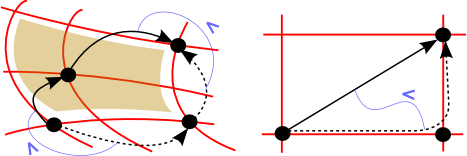
\includegraphics[bb=0 0 374 125]{imagenes/esquina.png}
  % esquina.png: 467x156 pixel, 90dpi, 13.18x4.40 cm, bb=0 0 374 125
  \label{fig:esquina}
  \caption{%
    Comparación entre la desigualdad de esquina y la desigualdad
    triangular.  La desigualdad triangular compara la distancias directa con
    la distancia a lo largo de dimensiones entre dos puntos.  La desigualdad de
    esquina sólo impone estas restricciones por tramos, pero deben cumplirse
    para cualquier lugar de la zona sombreada donde esté el punto central.
  }
\end{figure}


\end{document}
